\documentclass[tikz,border=10pt]{standalone}
\usepackage{tikz}
\usetikzlibrary{shapes.geometric}
\usetikzlibrary{angles,quotes,calc}

\begin{document}
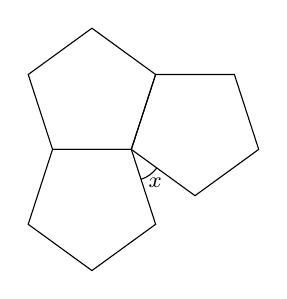
\begin{tikzpicture}[scale = 1]
    % Draw the original pentagon
    \coordinate (A) at (0,0);
    \draw (A) -- ++(180:1cm) coordinate (B) -- ++(108:1cm) coordinate(C) -- ++(36:1cm) coordinate (D) -- ++(-36:1cm) -- cycle;

%first rotated pentagon
\begin{scope}[rotate around={-108:(A)}]
    \draw (A) -- ++(180:1cm) coordinate (B) -- ++(108:1cm) coordinate(C) -- ++(36:1cm) coordinate (D) -- ++(-36:1cm) -- cycle;
\end{scope}

%second rotated pentagon
\begin{scope}[rotate around={-252:(A)}]
    \draw (A) -- ++(180:1cm) coordinate (B) -- ++(108:1cm) coordinate(C) -- ++(36:1cm) coordinate (D) -- ++(-36:1cm) -- cycle;
\end{scope}

\path (A) -- ++(-36:1cm) coordinate (K);
\path (A) -- ++(-72:1cm) coordinate (L);

\pic [draw, "\footnotesize $x$", angle eccentricity=1.3, angle radius=0.4cm] {angle = L--A--K};


\end{tikzpicture}
\end{document}`